
\documentclass{beamer}

\graphicspath{{./figure/}}

\usepackage[labelformat=empty,font=footnotesize]{caption}

\usepackage{cmap}

\usepackage{minted}
\setminted{baselinestretch=1}

\usepackage{verbatim}

\usepackage[T2A]{fontenc}
\usepackage[lutf8x]{luainputenc}
\usepackage[russian,english]{babel}

\usepackage{color}

\usepackage{comment}

\usepackage[export]{adjustbox}

\usepackage{dblfloatfix}

\usepackage{tikz}
\usetikzlibrary{graphs,arrows,positioning,graphdrawing}
\usegdlibrary{trees,force,layered}

\usetheme{Madrid}
\usecolortheme{beaver}

\title[Идентификация и автодифф.]{
	Применение автоматического дифференцирования при параметрической идентификации
	стохастических непрерывно-дискретных моделей
}
 
%\subtitle{A short story}
 
\institute[НГТУ, ФПМИ, ТПИ]{
	Новосибирский государственный технический университет (НГТУ) \\
	Факультет прикладной математики и информатики (ФПМИ) \\
	Кафедра теоретической и прикладной информатики (ТПИ)
}

\author[Горбунов К.]{
	Горбунов Константин, \tiny{магистрант, гр. ПММ-61} \\ 
	e-mail: gorbunov.2011@stud.nstu.ru \\
	\normalsize{Руководитель: Черникова Оксана Сергеевна, \tiny{доцент кафедры ТПИ}}
}
 
\date[НТИ-2017]{
	XI Всероссийская научная конференция молодых ученых \\ 
	<<Наука. Технологии. Инновации>> \\
	4 декабря -- 8 декабря~2017~года
}

\begin{document}


\frame{\titlepage}


\section*{Содержание}

\begin{frame}{\secname}{\subsecname}
	\tableofcontents[pausesections,pausesubsections]
\end{frame}


\section{Введение}

\subsection{Об идентификации}

\begin{frame}{\secname}{\subsecname}
	Сферы: \pause
	\begin{itemize}
	  \item наука, техника \pause
	  \item экономика, финансы \pause
	\end{itemize}
	\medskip
	Смежные задачи: \pause
	\begin{itemize}
	  \item планирование идентификационного эксперимента \pause
	  \item оценивание состояния (фильтрация) \pause
	  \item прогнозирование \pause
	  %\item синтез (проектирование) % ?
	  \item управление \pause
	\end{itemize}
	\medskip
	Предполагается считать тему работы актуальной.
\end{frame}


\begin{frame}{\secname}{\subsecname}
  Идентификация \pause
  \begin{itemize}
	\item в широком смысле: \\ \pause
	  Структура модели неизвестна. \pause
	\medskip
	\item в узком смысле: \\ \pause
	  Структура модели известна с точностью до некоторых неизвестных
	  параметров.
  \end{itemize}
\end{frame}


\section{Автоматическое дифференцирование (АД)}

\subsection{Предпосылки создания и применения метода АД}

\begin{frame}{\secname}{\subsecname}
	Для иллюстрации АД рассмотрим задачу идентификации в широком смысле. \\
	\pause

  Алгоритм идентификации: \pause
  \begin{enumerate}
	\item выбор структуры модели \pause
	\item оценивание параметров \pause
	\begin{itemize}
	  \item выбор критерия идентификации (ММП, МНК или др.) \pause
	  \item выбор алгоритма оценивания отклика (и состояния) \pause\\(фильтр Калмана
		или его модификация) \pause
	  \item программирование вычисления критерия \pause
	  \item программирование вычисления градиента критерия \pause
	\end{itemize}
	\item проверка модели на адекватность: если адекватна, закончим процесс,
	  иначе вернуться к выбору структуры модели
  \end{enumerate}
  
\end{frame}

\begin{frame}{\secname}{\subsecname}
  Рассмотрим этап программирования вычисления градиента критерия. \pause
  \begin{enumerate}
	\item вывод аналитического выражения градиента критерия \pause (либо применить
	  конечно-разностный численный метод и закончить процесс) \pause
	\item (непосредственно) программирование вычислений
  \end{enumerate}
\end{frame}

\begin{frame}{\secname}{\subsecname}
  Варианты: \pause
  \begin{itemize}
	\item каждый раз выводить аналитически новый градиент, \pause переписывать
	процедуру вычисления градиента критерия \pause
  \item хранить процедуры вычисления градиентов <<на все случаи жизни>> \pause
  \end{itemize}
  DRY --- Don't Repeat Yourself. \\ \pause
  Альтернатива: автоматическое дифференцирование
\end{frame}

\begin{frame}{\secname}{\subsecname}
  \begin{figure}
	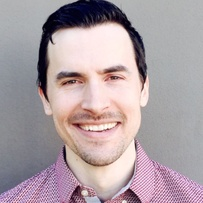
\includegraphics[width=0.2\textwidth,left]{domke-headshot}
	\caption{
	  Justin Domke \\
	  Assistant Professor \\
	  College of Computing and Information Sciences \\
	  University of Massachusetts, Amherst
	}
  \end{figure} \pause
	В 2009 году написал в своём блоге статью с названием \pause <<Automatic
	Differentiation: The most criminally underused tool in the potential machine
	learning toolbox?>>
  --- <<Автоматическое дифференцирование: наиболее пренебрегаемый
  инструмент в потенциальном арсенале исследователя \ldots>>.
\end{frame}


\subsection{Описание, определение}

\begin{frame}{\secname}{\subsecname}
  Автоматическое дифференцирование \pause
  \begin{itemize}
	\item основано на представлении функции как суперпозиции элементарных
	  функций и арифметических операций, каждая из которых дифференцируема и
	  производная известна \pause
	\item основано на правиле дифференцирования сложной функции (<<правиле
	  цепи>> --- <<chain-rule>>) \pause
	\item особенно актуально для обучения нейронных сетей (особенно глубинных, с
		десятками-сотнями тысяч, миллионами параметров)
  \end{itemize}
\end{frame}


\subsection{Иллюстрация}

\begin{frame}{\secname}{\subsecname}
	\begin{figure}[H]
	\raggedright
	\begin{minipage}{.5\textwidth}
	\begin{tikzpicture}[
			remember picture,overlay,
			>=stealth',
			node distance=10mm and 10mm,
			op/.style={
				draw,
				rectangle,
				minimum size=6mm,
				rounded corners=3mm
			}
		]
		\tikz[overlay,remember picture]
		\graph[layered layout,grow'=right,branch down=7mm] {
			{
				t/{$t$}, 
				w/{$\omega$}
			} ->
			wt/{$\cdot$} [op] -> sin/{$\sin$} [op]
				-> a1sin/{$\cdot$} [op] -> plus/{$+$} [op];
			a1/{$a_1$} -> a1sin;
			a0/{$a_0$} -> plus -> "$a_0 + a_1 \sin(\omega t)$";

			dt/{$t'$} ->[dashed] wdt/{$\cdot$} [op];
			w ->[dashed] wdt;
			dw/{$\omega'$} ->[dashed] tdw/{$\cdot$} [op]; 
			t ->[dashed] tdw;
			tdw ->[dashed] dwt/+[op,right=5mm of tdw];
			wdt ->[dashed] dwt;
			wt ->[dashed] cos/{$\cos$} [op];
			cos ->[dashed] dsin/{$\cdot$}[op];
			dwt ->[dashed] dsin;
			sin ->[dashed] sinda1/{$\cdot$}[op];
			da1/{$a_1'$} ->[dashed] sinda1 -> da1sin/+[op];
			dsin ->[dashed] a1dsin/{$\cdot$}[op];
			a1 ->[dashed] a1dsin;
			a1dsin -> da1sin;
			da0/{$a_0'$} ->[dashed] da0a1sin/+[op];
			da1sin ->[dashed] da0a1sin ->[dashed] "$(a_0 + a_1 \sin(\omega t))'$";
		};
	\end{tikzpicture}
	\end{minipage}
	\end{figure}
\end{frame}


\subsection{Доступные программные инструменты}

\begin{frame}[fragile]{\secname}{\subsecname}
	\begin{itemize}
		\item Python: autograd 
		\medskip
		\begin{minted}{python}
		import autograd.numpy as np
		from autograd import grad

		def f(x):
		    # your numpy function
		    pass

		grad_f = grad(f)
		# call grad_f()
		\end{minted}
		\medskip
		\item Python: TensorFlow
	\end{itemize}
\end{frame}


\section{Постановка задачи}

\subsection{Описание модельной структуры}

\begin{frame}{\secname}{\subsecname}
Рассмотрим модель стохастической динамической линейной непрерывно-дискретной
системы в простанстве состояний в общем виде:
\begin{equation}
	\label{eq:initmod}
	\left\{ 
		\begin{array}{lll}
			\frac{d}{dt}\vec{x}(t) &= F \vec{x}(t) + C \vec{u}(t) + G \vec{w}(t),
				& t \in [t_0,T] \\ 
			\vec{y}(t_k)           &= H \vec{x}(t_k) + \vec{v}(t_k), 
				& k = 1,\ldots, N
		\end{array} 
	\right. 
\end{equation}

\end{frame}

\subsection{Критерий идентификации}

\newcommand{\eps}{\varepsilon}

\begin{frame}{\secname}{\subsecname}
Критерий идентификации --- критерий максимального правдоподобия.
\begin{equation}
\begin{split}
\chi(\theta) = -\ln{L(Y_1^N;\theta)} = \frac{Nm}{2} \ln{2\pi} +
\\ + \frac{1}{2} \sum\limits_{k=1}^{N} 
\left[ \eps^T(t_k, \theta) B^{-1}(t_k, \theta) \eps(t_k, \theta) + 
\ln \det B(t_k, \theta) \right].
\end{split}
\end{equation}
\end{frame}


\section{Результаты исследований}

\begin{frame}
	Для различных случаев вхождения параметров в компоненты модели в
	результате проведения процедуры идентификации с использованием АД были
	получены оценки параметров по точности сопоставимые с результатами,
	полученными с использованием аналитического выражения градиента критерия.
\end{frame}

\section{Дальнейшие планы исследований}


\begin{frame}{\secname}
	Применить АД к модели, уравнение эволюции которой задано неявно, то есть и
	имеет вид: 
	\[
		f(\dot{x},x,w,u,t,\theta)=0,
	\]
	откуда невозможно явно выразить $\dot{x}$.
\end{frame}

\begin{frame}
\begin{center}
  \LARGE{Спасибо за внимание.}
\end{center}
\end{frame}

\begin{frame}[allowframebreaks]
	\frametitle{Литература}
\begin{thebibliography}{9}

% FIXME: fix to conform with GOST

\bibitem{denisov} Активная параметрическая идентификация стохастических
линейных систем: монография / В.И. Денисов, В.М. Чубич, О.С. Черникова, Д.И.
	Бобылева. --- Новосибирск : Изд-во НГТУ, 2009. --- 192 с.
	\mbox{(Серия <<Монографии НГТУ>>)}.

\bibitem{chubich} Активная параметрическая идентификация стохастических
	динамических систем. Оценивание параметров: учеб. пособие / В.М. Чубич,
	\mbox{Е.В. Филиппова}. --- Новосибирск: Изд-во НГТУ, 2016. --- 63 с.

\bibitem{colah} Chris Olah. ''Calculus on Computational Graphs:
Backpropagation'', colah's blog. August 31, 2015.
URL: colah.github.io/posts/2015-08-Backprop

\bibitem{ad-ml-survey} A. Baydin, B. Pearlmutter, A. Radul, J. Siskind.
Automatic Differentiation in Machine Learning: a Survey. {arXiv:0706.1234 [cs.SC]}

% плохое оформление библиографии или плохой источник?
\bibitem{tf} Martín Abadi, Ashish Agarwal, Paul Barham, et al.
TensorFlow: Large-scale machine learning on heterogeneous systems,
2015. Software available from tensorflow.org. {arXiv:1603.04467 [cs.DC]}

\bibitem{theano} J. Bergstra, O. Breuleux, F. Bastien, et al. “Theano: A CPU
and GPU Math Expression Compiler”. Proceedings of the Python for Scientific
Computing Conference (SciPy) 2010. June 30 - July 3, Austin, TX

\bibitem{torch} Collobert, Ronan, Koray Kavukcuoglu, and Clément Farabet.
"Torch7: A matlab-like environment for machine learning." BigLearn, NIPS
Workshop. No. EPFL-CONF-192376. 2011.

\end{thebibliography}
\end{frame}



\frame{\titlepage}

\end{document}
